\documentclass[a4paper, 12pt]{article}
\usepackage[utf8]{inputenc}
\usepackage[russian]{babel}
\usepackage{graphicx}
\usepackage{amsmath}
\usepackage[hidelinks]{hyperref}
\usepackage{minted}
\usepackage{indentfirst}
\usepackage{booktabs}

% Настройки minted
\setminted{fontsize=\footnotesize, linenos, breaklines, frame=single}

\begin{document}

% Title Page
\begin{titlepage}
    \centering
    {\Large МИНОБРНАУКИ РОССИИ \par}
    {\large Федеральное государственное бюджетное образовательное учреждение высшего образования\par}
    {\large САРАТОВСКИЙ НАЦИОНАЛЬНЫЙ ИССЛЕДОВАТЕЛЬСКИЙ ГОСУДАРСТВЕННЫЙ УНИВЕРСИТЕТ ИМЕНИ Н. Г. ЧЕРНЫШЕВСКОГО\par}
    \vspace{2cm}
    {\large Кафедра математической кибернетики и компьютерных наук\par}
    \vspace{3cm}
    {\LARGE \textbf{Реферат на тему:}\par}
    {\LARGE \textbf{«IT - специалист будущего»}\par}
    \vspace{3cm}
    \begin{flushright}
        Выполнил студент 1 курса 111 группы\\
        Индюков Кирилл Дмитриевич\\
        \vspace{1cm}
        Научный руководитель:\\
        к.п.н. доцент А.П. Грецова
    \end{flushright}
    \vspace{2cm}
    {\large Саратов\\2024}
\end{titlepage}

% Table of Contents
\tableofcontents
\newpage

% Sections
\section*{Введение}
\addcontentsline{toc}{section}{Введение}
В современном мире информационные технологии играют ключевую роль в различных сферах деятельности человека. Благодаря постоянному развитию и инновациям в этой области возникают новые перспективы и возможности как для бизнеса, так и для обычных пользователей. Именно поэтому изучение технологий будущего для ИТ-специалистов становится все более актуальным и востребованным.

В данной работе мы рассмотрим несколько ключевых аспектов, связанных с будущим информационных технологий. Во-первых, мы проанализируем востребованность ИТ-специалистов в будущем, исходя из современных тенденций и прогнозов развития отрасли. Во-вторых, мы изучим влияние IT-технологий на мировые экономические процессы и бизнес-среду в целом.

Особое внимание будет уделено трендам развития технического прогресса, таким как искусственный интеллект, интернет вещей (IoT), блокчейн технологии и кибербезопасность. Мы рассмотрим перспективы развития этих технологий и их воздействие на будущее, а также роль, которую они будут играть в цифровой трансформации общества.

Кроме того, будут рассмотрены вопросы образования и подготовки ИТ-специалистов на будущее, учитывая изменяющиеся требования рынка труда и технологические инновации. Наконец, мы коснемся этических аспектов применения IT-технологий в будущем, их влияния на общество и необходимости разработки соответствующих норм и правил использования новых технологий.

Таким образом, данная работа позволит более глубоко проанализировать перспективы развития информационных технологий и их влияние на различные сферы жизни, а также подготовиться к вызовам и возможностям, которые представляет собой будущее в области IT.

\section{Востребованность ИТ-специалистов в будущем}
\subsection{Будущие IT-профессии}
В настоящее время IT продолжает оставаться одной из самых быстрорастущих сфер экономики. Глобальный тренд на цифровизацию и все большее проникновение digital-продуктов в нашу жизнь заставляют развиваться и рынок труда, создавая все больше новых профессий.

Новые цифровые специальности создают пространство для маневра. Усложнение работы digital-систем, распространенность технологий с искусственным интеллектом и облачных хранилищ рождает спрос на профессии на стыке программирования, аналитики и больших данных.

\subsection{Тенденции развития отрасли}
Современные тенденции показывают, что рынок труда будет нуждаться в специалистах, способных работать с большими данными, развивать и поддерживать системы искусственного интеллекта, заниматься кибербезопасностью и управлять IT-инфраструктурой компаний.

\section{Тренды развития технического прогресса и их влияние на IT специальности}
\subsection{Искусственный интеллект: перспективы развития}
Искусственный интеллект (ИИ) представляет собой одну из самых перспективных и быстро развивающихся областей IT. В будущем ИИ будет играть ключевую роль в автоматизации процессов, анализе данных и принятии решений. 

Пример формулы, описывающей работу нейронной сети:
\begin{equation}
    y = \sigma(Wx + b)
    \label{eq:neural_network}
\end{equation}
где \( y \) -- выход, \( x \) -- входные данные, \( W \) -- матрица весов, \( b \) -- смещение, \( \sigma \) -- функция активации.

\subsection{Интернет вещей (IoT)}
Интернет вещей становится все более распространенным, объединяя в единую сеть различные устройства и системы. Это открывает новые возможности для мониторинга, управления и оптимизации различных процессов. 

Пример формулы для расчета количества подключенных устройств в сети IoT:
\begin{equation}
    N = \frac{B \cdot R}{P}
    \label{eq:iot_devices}
\end{equation}
где \( N \) -- количество устройств, \( B \) -- пропускная способность, \( R \) -- скорость передачи данных, \( P \) -- средний объем данных на одно устройство.

\subsection{Блокчейн технологии}
Блокчейн технологии находят свое применение не только в финансовой сфере, но и в других отраслях, требующих высокой степени безопасности и прозрачности данных. 

Пример формулы для вычисления хеш-функции:
\begin{equation}
    h = H(m)
    \label{eq:blockchain_hash}
\end{equation}
где \( h \) -- хеш, \( H \) -- хеш-функция, \( m \) -- сообщение.

\subsection{Кибербезопасность}
С ростом цифровизации и увеличением количества данных, кибербезопасность становится критически важной областью. Защита данных и предотвращение кибератак будут ключевыми задачами для будущих IT-специалистов.

Пример кода на Python для шифрования данных:
\begin{minted}{python}
from cryptography.fernet import Fernet

# Генерация ключа
key = Fernet.generate_key()
cipher_suite = Fernet(key)

# Шифрование сообщения
message = b"Confidential data"
cipher_text = cipher_suite.encrypt(message)
print(cipher_text)

# Расшифровка сообщения
plain_text = cipher_suite.decrypt(cipher_text)
print(plain_text)
\end{minted}

\section{Образование и подготовка ИТ-специалистов}
Для успешной карьеры в IT необходимо постоянное обновление знаний и навыков. Вузы и образовательные центры должны адаптировать свои программы к быстро меняющимся требованиям рынка труда.

\section{Этические аспекты применения IT-технологий}
Внедрение новых технологий неизбежно вызывает вопросы этики. IT-специалисты должны учитывать влияние своих разработок на общество и придерживаться этических норм.

\section{Заключение}
Информационные технологии продолжают оказывать значительное влияние на все аспекты нашей жизни. Будущее IT представляется как эра инноваций, где новые технологии будут постоянно преобразовывать мир вокруг нас. 

Подготовка квалифицированных специалистов, способных эффективно работать с новыми технологиями, является ключом к успешному развитию этой области. Этичные аспекты и безопасность также должны занимать важное место в процессе разработки и внедрения IT-решений.
    \section{Часть которя нужна как обязатльное требование}

    \begin{equation}
    y(x)=
        \begin{cases}
            x, ~ \text{если} ~ x>5
            \\
            5, | \text{иначе}
        \end{cases}
\end{equation}

Выносная формула 
\begin{equation}
    \alpha^{y^b}_{b+4}
    \max(x,y)
\end{equation}

\label{eq:strange}
\subsection{ формулы}
    \begin{equation}
    f(x)=\sum{n+1}
    \end{equation}

  формула  $y=x^2_1$


матрицы
    \begin{equation}
    X=
        \begin{Vmatrix}
        0 & 1 & 2 \\
        2 & 2 & 3 \\
        7 & 2 & 5 \\
        \end{Vmatrix}
    \end{equation}
% Пример изображения
\begin{figure}[h!]
    \centering
    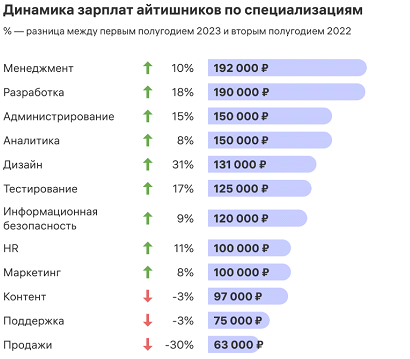
\includegraphics[width=0.5\textwidth]{Picthers/example_image1.png}
    \caption{Пример изображения 1}
    \label{fig:image1}
\end{figure}


% Пример второго изображения
\begin{figure}[h!]
    \centering
    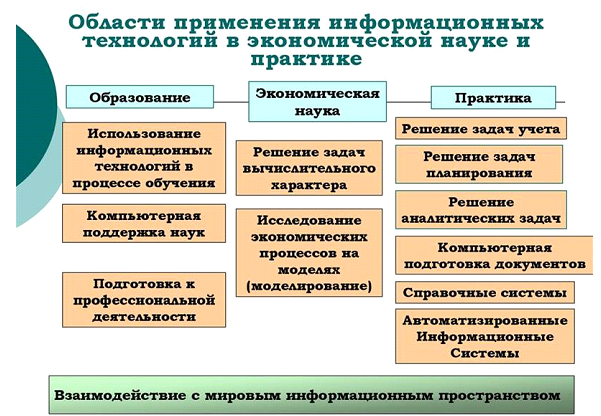
\includegraphics[width=0.5\textwidth]{Picthers/example_image2.png}
    \caption{Пример изображения 2}
    \label{fig:example_image2.png}
\end{figure}

% Пример таблицы
\begin{table}[h!]
    \centering
    \begin{tabular}{lrr}
        \toprule
        \textbf{Название} & \textbf{Значение 1} & \textbf{Значение 2} \\
        \midrule
        Строка 1 & 10 & 20 \\
        Строка 2 & 30 & 40 \\
        Строка 3 & 50 & 60 \\
        \bottomrule
    \end{tabular}
    \caption{Пример таблицы}
    \label{tab:example_table}
\end{table}

\newpage


\addcontentsline{toc}{section}{Список литературы}

% Отобразить все источники, даже те, на которые нет ссылок.
\nocite{*}

\bibliographystyle{ugost2003}
\bibliography{graph}

\end{document}
